\documentclass[11pt]{article}
\usepackage[margin=1in]{geometry}
\usepackage{amsmath,amssymb,amsthm}
\usepackage{graphicx}
\usepackage{xcolor}
\usepackage{booktabs}
\usepackage[numbers,sort&compress]{natbib}
\usepackage[colorlinks=true,linkcolor=blue!50!black,citecolor=blue!50!black,urlcolor=blue!50!black]{hyperref}

\newtheorem{theorem}{Theorem}
\newtheorem{lemma}{Lemma}
\newtheorem{corollary}{Corollary}
\theoremstyle{remark}
\newtheorem{remark}{Remark}

\newcommand{\Hhat}{\hat{H}}
\newcommand{\Vhat}{\hat{V}}
\newcommand{\dd}{\mathrm{d}}
\newcommand{\Ind}[1]{[\,#1\,]}

\title{The instability of negative-mass Schwarzschild\\is a point-mass effect:\\[4pt]
\large Exact thresholds for finite stars and a radially stable negative-mass boson star}
\author{Nathan Moinvaziri\thanks{\href{mailto:nathan@nathanm.com}{nathan@nathanm.com}}\\[2pt]
\normalsize\textit{Independent researcher}}
\date{October 2026}

\begin{document}
\maketitle

\begin{abstract}
Negative-mass Schwarzschild spacetime is linearly unstable: Gleiser and Dotti exhibited, for every multipole
$\ell\ge2$, an even-parity mode growing as $e^{\gamma t}$ with $\gamma=(\ell-1)\ell(\ell+1)(\ell+2)/(12|M|)$, and
gave numerical evidence that it is the only one. It has been suggested that the instability does not depend on the
singularity and would survive in a regular negative-mass star. We prove, for every $\ell\ge2$, that the
Dotti--Gleiser operator has exactly one negative eigenvalue. The proof uses the zero-energy partner solution
$\phi_0=1/\psi_0$ implicit in their intertwining construction, through a ground-state identity and Glazman's lemma.
The same identity yields an exact count of unstable modes for the exterior of a star of areal radius $R$ whose
interior imposes a Robin condition $\hat\Psi'=\kappa\hat\Psi$:
$\#\{\gamma>0\}=\Ind{R<r_s}+\Ind{\kappa<\kappa_c(R)}$, with $r_s=6|M|/[(\ell+2)(\ell-1)]$ and $\kappa_c$ in closed form.
Consequently the vacuum exterior of any star with $R\ge r_*(\ell)$ ($r_*=2.279|M|$ for $\ell=2$) and a
non-energy-injecting surface condition ($\kappa\ge0$) supports no unstable even-parity mode, and the $\ell^4$ growth
of the point mass is capped by any finite radius. We then study a concrete regular negative-mass object, a sextic boson star whose stress tensor enters
Einstein's equations with a minus sign. We derive its radial perturbation equations, verify them symbolically, and
find the configuration used in a recent full numerical-relativity study to be radially stable; the family loses
stability exactly where the Noether charge is extremal. Because the first law becomes $\dd M=-\omega\,\dd N$, the
turning-point criterion holds in $N$ but reverses sign when written in $M$. Accurate spherically symmetric nonlinear
evolutions confirm both the stationarity of the stable stars to $t=1500$ and the predicted growth rates of unstable ones.
\end{abstract}

\section{Introduction}

Bondi's 1957 analysis~\cite{Bondi1957} showed that general relativity contains no logical obstruction to negative
mass, provided inertial, passive and active mass share a sign, and that a pair of equal and opposite masses
self-accelerates (the ``runaway''). Two questions have dominated the subsequent discussion: whether negative mass is
dynamically stable, and whether the runaway is physical. The second was recently addressed by full $3+1$ evolutions of a
canonical boson star paired with a ``phantom'' boson star of negative ADM mass~\cite{Shirokov2026}. Here we address the
first.

For the vacuum point mass the answer is known. Gibbons, Hartnoll and Ishibashi~\cite{GHI2005} proved stability of the
odd-parity sector and, for a range of boundary conditions at the naked singularity, of the even sector. Gleiser and
Dotti~\cite{GD2006} then found exact, smooth, exponentially growing even-parity solutions and showed that the stability
argument of Ref.~\cite{GHI2005} relies on a perturbation that is not continuous at an interior radius where the Zerilli
variable is singular. Dotti and Gleiser~\cite{DG2009} removed that ``kinematic'' singularity with an intertwining
operator, obtained a regular operator $\Hhat$ with a unique self-adjoint extension, and showed that the unstable mode is
excited by generic data supported away from the singularity. Cardoso and Cavagli\`a~\cite{CC2006} identified the modes as
algebraically special. Whether the unstable mode is the only one was left as numerical evidence~\cite{DG2009}.

What a regular negative-mass source does to this instability has not been computed. In a recent review Dotti suggests
that replacing the singularity by a small negative-mass distribution would leave the potential largely unchanged, so
that ``an unstable mode could be found anyway'', and that ``the singularity plays no role in the
instability''~\cite{Dotti2022}. Regular negative-mass configurations exist---perfect-fluid bubbles in de
Sitter~\cite{MP2014}, scalar-field stars~\cite{Shirokov2026}---but stability analyses have been radial and restricted to
special matter models~\cite{Johnson2020,Alves2025}.

This paper makes three contributions.
\begin{enumerate}
\item We prove that $\Hhat$ has exactly one negative eigenvalue for every $\ell\ge2$ (Theorem~\ref{thm:one}), turning
the numerical observation of Ref.~\cite{DG2009} into a theorem.
\item For the exterior of a star of radius $R$ with a Robin interface condition, we give an exact count of unstable modes
for every $\ell$ (Theorem~\ref{thm:trunc}). The instability is a property of the region $r\lesssim 10|M|/\ell^2$: a star
larger than $r_*(\ell)$ hides it unless its surface condition injects energy, and any finite star caps the growth rate.
This quantifies, and for dilute stars contradicts, the expectation of Ref.~\cite{Dotti2022}.
\item We give the first linear stability analysis of a negative-ADM-mass boson star~\cite{Shirokov2026}. It is radially
stable on the branch used in numerical relativity, with stability lost exactly at the extremum of the Noether charge.
\end{enumerate}
The non-radial stability of the boson star, which requires computing the effective interface condition that its
interior supplies, is left for future work (Sec.~\ref{sec:discussion}).

Units $G=c=1$. Sections~\ref{sec:op}--\ref{sec:trunc} use $|M|=1$; Sec.~\ref{sec:bs} uses the scalar mass $m=1$.
All computations are reproducible from the accompanying repository.

\section{The intertwined Zerilli operator}\label{sec:op}

Write the negative-mass Schwarzschild metric as $\dd s^2=-f\dd t^2+f^{-1}\dd r^2+r^2\dd\Omega^2$ with
$f=1-2M/r=1+2/r$ ($M=-1$), and the tortoise coordinate $x=r-2\ln(1+r/2)$, so $x\in(0,\infty)$ with $x\simeq r^2/4$ at
the singularity. Even-parity perturbations with multipole $\ell\ge2$ reduce to Zerilli's equation~\cite{Zerilli1970}
$\partial_t^2\Psi_Z+H_Z\Psi_Z=0$, $H_Z=-\partial_x^2+V_Z$. Let
\begin{equation}
c=(\ell+2)(\ell-1),\qquad k=\frac{(\ell-1)\ell(\ell+1)(\ell+2)}{6}=\frac{c(c+2)}{6},\qquad r_s=\frac{6}{c}.
\end{equation}
For $M<0$ the potential $V_Z$ has a double pole at $r_s$, which lies in the physical domain; it is ``kinematic'' because
$\Psi_Z$ itself has a simple pole there for smooth metric perturbations~\cite{GD2006}.

Dotti and Gleiser~\cite{DG2009} use the static solution $\psi_0=\chi(r)/(cr-6)$ of $H_Z\psi_0=0$, where $\chi$ is the
polynomial of degree $\ell+2$ in their Eq.~(55), and define $g=\psi_0'/\psi_0$ ($'=\dd/\dd x$),
\begin{equation}
A=\partial_x+g,\qquad H_Z=AA^*,\qquad \Hhat=A^*A=-\partial_x^2+\Vhat,\qquad \Vhat=g^2-g'.
\end{equation}
$\Vhat$ is regular, $\Hhat A^*=A^*H_Z$, and $\hat\Psi=A^*\Psi_Z$ is smooth for smooth metric perturbations. The
zero-energy partner of this factorisation,
\begin{equation}
\phi_0=\frac{1}{\psi_0}=\frac{cr-6}{\chi(r)},\qquad A\phi_0=0,\qquad \Hhat\phi_0=0,
\end{equation}
appears in Ref.~\cite{DG2009} as the state ``missing in the spectrum'' of the supersymmetric partner. It is the object
on which everything below rests. Figure~\ref{fig:vhat} shows $\Vhat$: it is negative only on a thin shell just outside
$r_s$, and when lengths are scaled by $c$ and energies by $k^2$ the shell is nearly independent of $\ell$.

\begin{figure}[t]
\centering
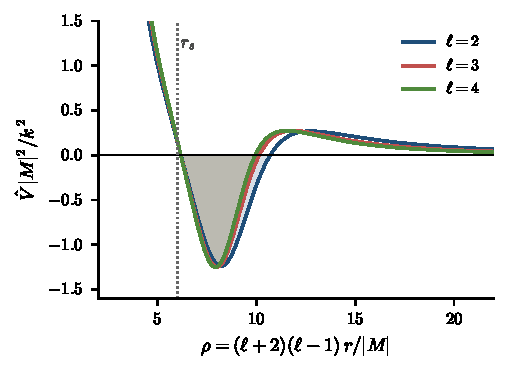
\includegraphics[width=0.48\textwidth]{figures/fig1_vhat.pdf}
\caption{The regularised potential $\Vhat$ for $\ell=2,3,4$, in the scaled radius $\rho=cr/|M|$. Shaded: $\Vhat<0$,
which occurs only on a shell just beyond $r_s$ ($\rho=6$). With radius scaled by $c=(\ell+2)(\ell-1)$ and the
potential by the eigenvalue scale $k^2$, the curves nearly coincide.}
\label{fig:vhat}
\end{figure}

\begin{lemma}[properties of $\chi$, $\phi_0$, $\Vhat$; all $\ell\ge2$]\label{lem:props}\leavevmode
\begin{enumerate}
\item $\chi=\sum_{n=1}^{\ell+2}c_n r^n$ with $c_1=\tfrac32$, $c_2=0$, $c_3=-K/32$, $c_4=K/96$ ($K=6k$), $c_n\ge0$ for
$n\ge4$ and $c_{\ell+2}>0$; $\psi_0$ solves the static Zerilli equation identically in $\ell$; and $\chi>0$ on $r>0$.
\item At $r_s$ the $\chi$-equation has Frobenius exponents $0$ and $3$, forcing $\chi''(r_s)=0$; hence $\Vhat$ is
real-analytic on $(0,\infty)$.
\item $r^4\Vhat=12+O(r)$ as $r\to0$ (exponents $x^{3/2}$, $x^{-1/2}$), and $\Vhat\simeq(\ell+1)(\ell+2)/r^2$ as
$r\to\infty$. $\Hhat$ is limit point at both ends, hence essentially self-adjoint on $C_c^\infty(0,\infty)$.
\item $\phi_0$ is the non-admissible branch $\propto x^{-1/2}$ at $0$, decays as $r^{-(\ell+1)}$ at infinity, and has
exactly one zero, at $r_s$, which is simple.
\end{enumerate}
\end{lemma}
\begin{proof}[Sketch]
(1) The closed form $c_n=(n-2)\bigl((n-4)\ell(\ell+1)+n-1\bigr)(\ell-n+3)_{2n-4}/\bigl(2^n(n-1)!^2\bigr)$ turns the static
equation into a three-term recurrence, which becomes a polynomial identity in $(\ell,n)$ after dividing by a Pochhammer
factor; it is verified symbolically. Positivity follows Ref.~\cite{DG2009}, Eqs.~(57)--(59): dropping the non-negative
terms $n\ge6$ leaves a quartic whose unique positive critical value is
$4(K-18)(Ks-18(K-16))/[(\ell-2)(\ell+3)(\ell^2+\ell+4)]^3$, $s=\sqrt{6(K-18)}$, which is positive because
$(Ks)^2-(18(K-16))^2=6(K-24)^3>0$ for $\ell\ge3$; $\ell=2$ is checked directly. (2)--(4) are local expansions, verified
symbolically in $\ell$; limit point at $0$ holds because $x^{-1/2}\notin L^2$, and the Weyl alternative gives essential
self-adjointness~\cite{ReedSimon2,Weidmann1987}.
\end{proof}

\section{Exactly one unstable mode}\label{sec:one}

The key tool is the ground-state identity: if $\Vhat=\phi_0''/\phi_0$ and $u=\phi_0 h$, then
\begin{equation}\label{eq:gs}
u'^2+\Vhat u^2=\phi_0^2h'^2+\bigl(\phi_0\phi_0'h^2\bigr)'.
\end{equation}

\begin{theorem}\label{thm:one}
For every $\ell\ge2$, $\Hhat$ has exactly one negative eigenvalue. It is simple and equals $-(k/2)^2$, so the unique
unstable even-parity mode of negative-mass Schwarzschild grows at the Gleiser--Dotti rate $\gamma=k/(2|M|)$. Zero is
not an eigenvalue.
\end{theorem}

\begin{proof}
\emph{At most one.} By Glazman's lemma~\cite{BirmanSolomyak}, the number of negative eigenvalues equals the largest
dimension of a subspace of a form core on which $q[u]=\langle u,\Hhat u\rangle$ is negative definite. Take the core
$C_c^\infty(0,\infty)$ and suppose such a subspace $F$ has $\dim F\ge2$. Choose $u\in F\setminus\{0\}$ with $u(x_s)=0$,
$x_s=x(r_s)$. Since $\phi_0$ is analytic with a simple zero at $x_s$, $h=u/\phi_0$ is smooth, and integrating
\eqref{eq:gs} over the compact support of $u$ gives $q[u]=\int\phi_0^2h'^2\,\dd x\ge0$, a contradiction.

\emph{At least one.} The function $\hat\Psi=A^*\Psi_{\rm DG}$, with
$\Psi_{\rm DG}=r(r+2)^ke^{-kr/2}/(cr-6)$, satisfies $\Hhat\hat\Psi=-(k/2)^2\hat\Psi$ identically in $\ell$, is
$O(r^3)$ at $0$, regular at $r_s$, and decays exponentially; so it is an eigenfunction. Independently of this explicit
mode, $w=\phi_0\mathbf 1_{x>x_s}$ lies in the form domain with $q[w]=0$ by \eqref{eq:gs}; if $\Hhat\ge0$, $w$ would be a
minimiser and hence a weak, therefore $C^1$, solution of $\Hhat w=0$, contradicting the kink at $x_s$.

\emph{No zero mode.} The zero-energy solution admissible at $x=0$ is
\[
v=\phi_0F,\qquad F(r)=\mathrm{f.p.}\!\int_0^r\psi_0^2\,\frac{\dd x}{\dd r}\,\dd r ;
\]
it grows as $r^{\ell+2}$ and is not in $L^2$.
\end{proof}

\begin{remark}
$v$ has exactly one zero for every $\ell$ ($F$ is positive on $(0,r_s)$ and increases from $-\infty$ to $+\infty$ on
$(r_s,\infty)$), as renormalised oscillation theory~\cite{GST1996} requires. The proof does not use oscillation theory at
the continuum edge. Numerically, Chebyshev discretisations with $\hat\Psi=r^3u$ reproduce $E_0=-(k/2)^2$ to
$\le3\times10^{-13}$ for $\ell\le8$ and find no second bound state in 140 resolution and domain variations.
\end{remark}

\section{Finite stars: an exact count}\label{sec:trunc}

Model the exterior of a star of areal radius $R$ by $\Hhat_{R,\kappa}$ on $L^2(x_R,\infty)$ with the Robin condition
$\hat\Psi'(x_R)=\kappa\hat\Psi(x_R)$; $\kappa=+\infty$ denotes Dirichlet. The interior matter determines $\kappa$, which in
general depends on frequency and $\ell$; here it is a free parameter. Define
\begin{equation}\label{eq:kc}
\kappa_c(R)=\frac{\dd\ln\phi_0}{\dd x}\Big|_R=\Bigl(1+\frac2R\Bigr)\frac{\mathcal N(R)}{(cR-6)\chi(R)},
\qquad \mathcal N=c\chi-(cr-6)\chi'.
\end{equation}

\begin{theorem}\label{thm:trunc}
For every $\ell\ge2$ and $R\neq r_s$, the number of negative eigenvalues of $\Hhat_{R,\kappa}$ is
\begin{equation}
\Ind{R<r_s}+\Ind{\kappa<\kappa_c(R)},
\end{equation}
with Dirichlet counted as $\kappa=+\infty$. At $\kappa=\kappa_c$, $\phi_0$ is a zero-energy eigenfunction.
\end{theorem}

\begin{proof}
For $u$ in the core, \eqref{eq:gs} gives $q[u]=\int\phi_0^2h'^2\,\dd x+(\kappa-\kappa_c)u(x_R)^2$ provided $u(x_s)=0$ when
$R<r_s$. Imposing $u(x_s)=0$ (if $R<r_s$) and $u(x_R)=0$ (if $\kappa<\kappa_c$) costs at most
$\Ind{R<r_s}+\Ind{\kappa<\kappa_c}$ linear conditions and leaves $q\ge0$; Glazman's lemma gives the upper bound. For the
lower bound use $w_1=\phi_0\mathbf 1_{[x_R,x_s]}$ and $w_2=\phi_0\mathbf 1_{[x_s,\infty)}$ (or $\phi_0$ itself if
$R>r_s$), for which $q[aw_1+bw_2]=a^2\phi_0(x_R)^2(\kappa-\kappa_c)$ and $q[w_2]=0$. If the negative spectral subspace
were smaller, some combination orthogonal to it would have $q=0$, hence be a weak zero-energy solution satisfying the
boundary condition; the kink of $w_2$, or $\kappa\ne\kappa_c$, excludes this.
\end{proof}

\begin{corollary}[thresholds, all $\ell$]\label{cor:thr}
$\mathcal N>0$ on $[0,r_s]$ and has exactly one root $r_*>r_s$. Hence $\kappa_c<0$ on $(0,r_s)$, $\kappa_c\to\mp\infty$
at $r_s^\mp$, $\kappa_c>0$ on $(r_s,r_*)$ and $\kappa_c<0$ on $(r_*,\infty)$. In particular:
Dirichlet is unstable iff $R<r_s$; Neumann is unstable iff $R<r_*$; every $\kappa\ge0$ is stable iff $R\ge r_*$.
\end{corollary}

The first claim follows from a telescoping lower bound on $[0,r_s]$; uniqueness of $r_*$ from Descartes' rule applied to
$\mathcal N(r_s+t)$, whose coefficients have one sign change because $\chi''(r_s)=0$ and $\chi^{(m)}(r_s)>0$ for
$m\ge4$. Table~\ref{tab:thr} lists the thresholds and Fig.~\ref{fig:kc} the critical surface condition. Asymptotically,
\begin{align}
\kappa_c&=-\frac{\ell+1}{R}-\frac{\ell^4+3\ell^3+4\ell^2+4}{\ell(\ell-1)(\ell+2)}\frac{1}{R^2}+O(R^{-3})
&&(R\to\infty),\\
\kappa_c\,x_R&=-\frac12-\frac{(\ell^2+\ell-1)R}{12}+O(R^2)&&(R\to0).
\end{align}
For large $R$ an instability therefore requires a surface condition softer than the static vacuum tail
$\phi_0\propto r^{-(\ell+1)}$ by an $O(1)$ factor on the scale $1/R$. As $R\to0$ every condition with
$\kappa x_R>-\tfrac12$ (including Dirichlet and Neumann) reproduces the Dotti--Gleiser eigenvalue, with error scaling
roughly as $R^3$--$R^4$, so the self-adjoint extension of Ref.~\cite{DG2009} is the limit of a regular cutoff; compare
the scalar-wave analysis of Ref.~\cite{Giveon2004}.

\begin{table}[t]
\centering
\begin{tabular}{cccccc}
\toprule
$\ell$ & $r_s$ & $r_*$ & $r_{\rm neg}$ & $\gamma_{\rm DG}=k/2$ & $|M|/r_*$\\
\midrule
2 & 1.5000 & 2.2788 & 2.6741 & 2 & 0.439\\
3 & 0.6000 & 0.8789 & 1.0143 & 10 & 1.14\\
4 & 0.3333 & 0.4814 & 0.5519 & 30 & 2.08\\
5 & 0.2143 & 0.3073 & 0.3512 & 70 & 3.25\\
\bottomrule
\end{tabular}
\caption{Thresholds in units of $|M|$. $r_s$: Dirichlet threshold; $r_*$: Neumann and $\kappa\ge0$ threshold;
$r_{\rm neg}=\sup\{r:\Vhat<0\}$. Since $r_*$ decreases with $\ell$ (checked for $\ell\le80$), a star with
$|M|/R<0.439$ and $\kappa\ge0$ has no unstable even-parity mode for any $\ell$. At large
$\ell$, $r_*\approx8.486/c$ and $r_{\rm neg}\approx9.636/c$ (derived from the $\ell\to\infty$ limit of $c\,\chi(\rho/c)$, a
modified-Bessel closed form; convergence of the roots is not proven).}
\label{tab:thr}
\end{table}

\begin{figure}[t]
\centering
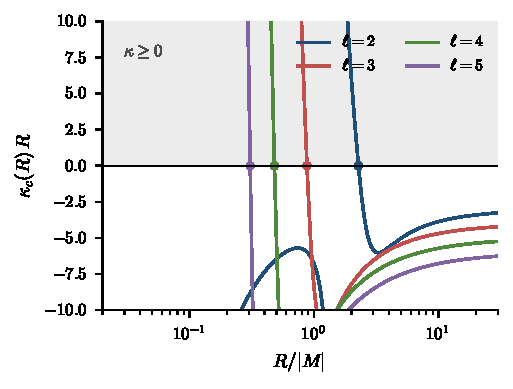
\includegraphics[width=0.48\textwidth]{figures/fig2_kappa_c.pdf}\hfill
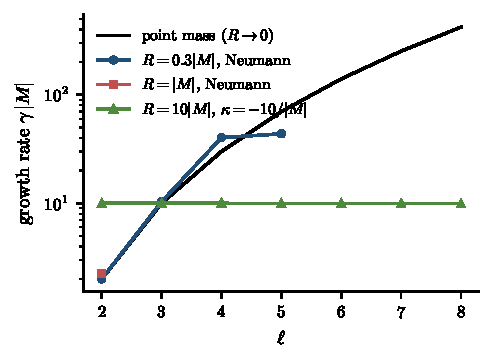
\includegraphics[width=0.48\textwidth]{figures/fig3_growth.pdf}
\caption{Left: critical surface condition $\kappa_c(R)R$ for $\ell=2$--$5$. A mode is unstable when $\kappa<\kappa_c$,
plus one unconditional mode when $R<r_s$ (pole). Dots mark $r_*$. Above $r_*$ the whole $\kappa\ge0$ region (shaded) is
stable. Right: growth rate versus $\ell$. The point mass grows as $\ell^4/12$; any finite $R$ with an $\ell$-independent
condition leaves finitely many unstable $\ell$ ($\kappa\ge0$) or caps the rate at $|\kappa|$ ($\kappa<0$, since
$\Vhat\ge0$ outside $r_{\rm neg}$).}
\label{fig:kc}
\end{figure}

\paragraph{Growth-rate cap.} For the point mass the growth rate $k/2\sim\ell^4/12$ is unbounded in $\ell$. For a star:
with $\kappa\ge0$ only $\ell$ with $R<r_*(\ell)$, roughly $\ell\lesssim3/\sqrt{R}$, are unstable; with a fixed $\kappa<0$,
every $\ell$ with $r_{\rm neg}(\ell)<R$ has $\Vhat\ge0$ outside the star and growth $\le|\kappa|$. Either way
$\sup_\ell\gamma<\infty$ (Fig.~\ref{fig:kc}, right; a 1000-case numerical scan agrees with Theorem~\ref{thm:trunc}).
The unbounded growth belongs to the singularity.

\section{A regular negative-mass star}\label{sec:bs}

Theorem~\ref{thm:trunc} reduces the even-parity stability of any star with $R>r_*$ to the sign of the effective $\kappa$
its interior supplies, together with the stability of the matter itself. We now examine the matter for a concrete
model.

\paragraph{Model.} Following Ref.~\cite{Shirokov2026}, take a complex scalar with
$\mathcal L=-\tfrac12|\nabla\Phi|^2-V(|\Phi|^2)$, $V(s)=\tfrac12s-\tfrac14\lambda s^2+\tfrac16\mu s^3$, $\lambda=10240$,
$\lambda^2/\mu=4.8$, coupled through
\begin{equation}
G_{ab}=8\pi\varepsilon\,T_{ab}[\Phi],\qquad \Box\Phi=2V'(|\Phi|^2)\Phi,
\end{equation}
with $\varepsilon=+1$ (canonical) or $\varepsilon=-1$. For $\varepsilon=-1$ the field equation is unchanged but the
star gravitates with negative ADM mass. In the language of Bondi, the scalar has a single mass parameter that is
inertial, passive and active at once, and is negative for $\varepsilon=-1$; gravity alone cannot distinguish this from
Bondi's ``all three negative''~\cite{Bondi1957,Bonnor1989}. The action is that of a ghost, so the model is a classical
probe; quantum mechanically it is unstable to vacuum decay~\cite{CJM2004}.

\paragraph{Static stars.} Stationary solutions $\Phi=\phi(r)e^{-i\omega t}$ in Schwarzschild-like coordinates are
solved as two-point boundary-value problems with a decaying Yukawa tail. The configuration of Ref.~\cite{Shirokov2026}
at $\omega=0.7603$ has $M=-0.014580$, rms radius $4.40$ and $|M|/R\approx3\times10^{-3}$, far below the threshold
$|M|/R<0.439$ of Table~\ref{tab:thr}: the shell where negative-mass Schwarzschild would be unstable lies deep inside the
matter. (Our masses are ADM masses; those quoted in Ref.~\cite{Shirokov2026} are the mass enclosed where $\phi$ falls to
$5\%$ of its central value and are $1.5$--$2.3\%$ smaller; the field profiles agree to $10^{-5}$.)

\paragraph{First law.} With $N=\int4\pi r^2\omega\phi^2(a/\alpha)\,\dd r$ the Noether charge, the family satisfies
\begin{equation}
\dd M=\varepsilon\,\omega\,\dd N,
\end{equation}
verified by finite differences to $<10^{-4}$. Hence $M(\omega)$ and $N(\omega)$ are extremal at the same $\omega$ for
either sign, but $\dd M/\dd\omega$ and $\dd N/\dd\omega$ have opposite signs when $\varepsilon=-1$.

\paragraph{Radial perturbations.} Perturbing the metric functions and both components of the field with
$e^{i\sigma t}$, we eliminate the metric through the $tr$ and $rr$ constraints and obtain a closed fourth-order system for
the real perturbation, a gauge-invariant phase and the perturbed enclosed charge, containing $\sigma$ only as $\sigma^2$
and $\varepsilon$ symbolically. Substituting back, all six linearised field equations are satisfied identically. The
structure is that of Refs.~\cite{GW1989,Kain2021}. Eigenvalues are found by compound-matrix shooting, which keeps the
two-dimensional space of decaying solutions well conditioned, and are cross-checked by an independent finite-difference
pencil that also returns complex eigenvalues.

\begin{figure}[t]
\centering
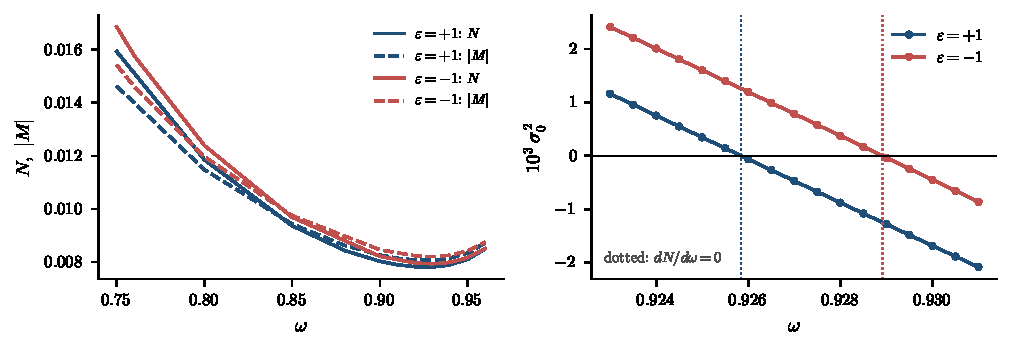
\includegraphics[width=0.97\textwidth]{figures/fig4_radial.pdf}
\caption{Radial stability of signed-source boson stars. Left: Noether charge $N$ and $|M|$ along the canonical
($\varepsilon=+1$) and phantom ($\varepsilon=-1$) families. Right: fundamental $\sigma_0^2$ near the stability change;
dotted lines mark $\dd N/\dd\omega=0$, which coincides with $\sigma_0^2=0$ to $2\times10^{-8}$ ($\varepsilon=+1$) and
$8\times10^{-8}$ ($\varepsilon=-1$) in $\omega$.}
\label{fig:radial}
\end{figure}

\paragraph{Results.} For $\varepsilon=+1$ the textbook criterion is reproduced at both turning points of the family: the
fundamental mode crosses zero at $\omega=0.92584444$ against $\dd M/\dd\omega=\dd N/\dd\omega=0$ at $0.92584446$, and
again at the strong-field maximum of $N$ ($\omega\approx0.200$, $N\approx42.73$) within the scan resolution. For
$\varepsilon=-1$ (Fig.~\ref{fig:radial}):
\begin{itemize}
\item The star of Ref.~\cite{Shirokov2026} is radially stable: no real growth rate up to $|\sigma|=2$ and no complex
eigenvalue with $|\sigma^2|<0.3$, at two resolutions of the finite-difference check.
\item The family is stable for $\omega<0.92891$ and unstable above. The crossing $\sigma_0^2=0$ at $\omega=0.92890846$
coincides with $\dd N/\dd\omega=0$ at $0.92890838$.
\item The criterion is therefore invariant when stated in $N$ (stable side $\dd N/\dd\omega<0$) but reverses when
stated in $M$: on the stable side $\dd M/\dd\omega=-\omega\,\dd N/\dd\omega>0$.
\item The phantom family has a fold in $\omega$ ($\omega_{\min}\approx0.4223$) at which neither $M$ nor $N$ is
extremal; the fundamental mode stays positive through it. The strong-field branch, followed to $|2m/r|\approx0.4$, is
stable with no turning point.
\end{itemize}
Near $\omega\approx0.93$ the instability is essentially the flat-space Vakhitov--Kolokolov instability of
$Q$-balls~\cite{Coleman1985,FLP1987}, with gravity a small correction; the strong-field branch is the more sensitive
test of how $\varepsilon$ enters. The first law and the $N$-form of the criterion follow from the standard turning-point
arguments~\cite{Sorkin1982,LeePang1989,KMS1991} with $\varepsilon$ kept; the new content is the explicit linear analysis
for $\varepsilon=-1$. The result is consistent with the theorem that barotropic negative-mass stars are radially
unstable~\cite{Alves2025}, which does not apply to scalar-field matter.

\paragraph{Nonlinear check.} We evolve single stars in spherical symmetry in polar-areal slicing, re-solving the
Hamiltonian constraint for the Misner--Sharp mass~\cite{MisnerSharp} and the slicing condition at every substep, with
$\varepsilon$ appearing only there~\cite{SeidelSuen1990,HawleyChoptuik2000}. The scheme is fourth order in space and time
and converges at order $\approx4$; the Misner--Sharp mass outside the star equals the ADM mass of the static solution to
$5\times10^{-8}$. Unstable stars at $\omega=0.94$, perturbed by $\pm\delta$, grow at $\sigma=0.07376$ ($\varepsilon=+1$)
and $0.06679$ ($\varepsilon=-1$) against $0.07370$ and $0.06668$ from the linear analysis (Fig.~\ref{fig:evol}, right).
The stable campaign stars of both signs remain stationary to $t=1500$, with fractional drifts of $\omega$, the central
amplitude, the Misner--Sharp mass and $N$ all $\le10^{-6}$ at $h=0.1$ and decreasing with resolution
(Fig.~\ref{fig:evol}, left). A $5\%$ perturbation relaxes within $\sim150$ time units onto the neighbouring static star
and stays there. The slow drifts reported for a lone phantom star in $3+1$~\cite{Shirokov2026} are therefore not a
property of the spherical dynamics.

\begin{figure}[t]
\centering
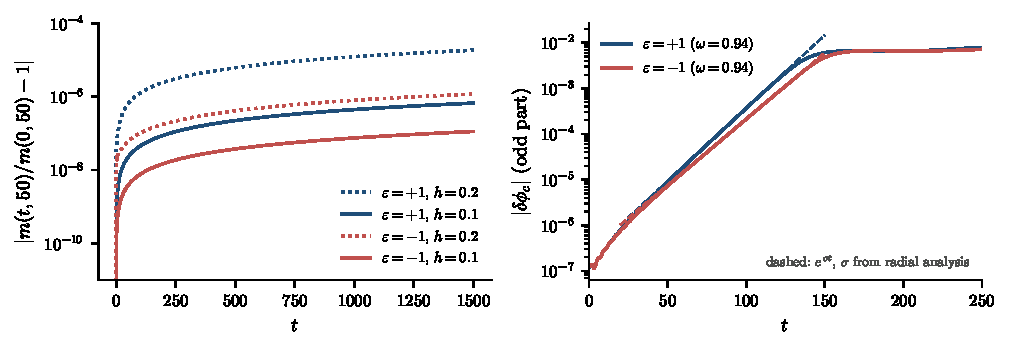
\includegraphics[width=0.97\textwidth]{figures/fig5_evolution.pdf}
\caption{Spherically symmetric nonlinear evolutions. Left: relative drift of the Misner--Sharp mass at $r=50$ for the
stable campaign stars ($\omega=0.750$ canonical, $\omega=0.7603$ phantom) at two resolutions; the drift is a
dissipation-limited truncation error that decreases rapidly with $h$. Right: odd part of the central-amplitude response
of unstable stars ($\omega=0.94$) to $\pm10^{-5}$ perturbations; dashed lines have the growth rates of the linear
analysis.}
\label{fig:evol}
\end{figure}

\section{Discussion}\label{sec:discussion}

For the point mass, Theorem~\ref{thm:one} completes the linear stability analysis of negative-mass Schwarzschild: one
unstable even-parity mode per $\ell$, at the Gleiser--Dotti rate, and no others. Theorem~\ref{thm:trunc} shows where that
mode lives. The negative part of the effective potential sits on a shell of radius $\approx10|M|/\ell^2$
(Fig.~\ref{fig:vhat}); a star whose surface lies outside $r_*(\ell)$ hides it unless its interior supplies an
energy-injecting surface condition, and for $\ell=2$ the condition is $|M|/R<0.439$. In this sense the instability is a
point-mass effect, contrary to the suggestion in Ref.~\cite{Dotti2022}: for a dilute regular source the vacuum exterior
cannot drive it, and the $\ell^4$ growth disappears.

What remains is a property of the matter. For the boson star of Ref.~\cite{Shirokov2026}, which is dilute
($|M|/R\sim10^{-3}$), we have shown radial stability. Non-radial stability requires the effective interface condition
$\kappa_{\rm eff}(\ell,\omega)$ produced by the interior, together with any instability intrinsic to the matter; the
polar perturbation equations of the signed-source boson star are the natural route, and we leave them for future work.
Theorem~\ref{thm:trunc} reduces the gravitational part of that question to a comparison of $\kappa_{\rm eff}$ with the
closed-form $\kappa_c(R)$.

Two limitations should be stated. Our results are classical: the phantom sector is a ghost, and a quantum theory of it
has an unstable vacuum~\cite{CJM2004}. And the Robin model of the interior is exact only for an interface condition
independent of frequency; a real star supplies a frequency-dependent one, for which Theorem~\ref{thm:trunc} gives the
count at each fixed frequency.

\section{How the results were obtained}\label{sec:method}

This work was carried out by the author working with an AI research assistant (Anthropic's Claude, run as an agent
with a Python environment and the ability to delegate independent tasks to parallel sub-agents). The author set the
questions, the scope and the priorities, and reviewed each stage; the assistant carried out the literature reading,
derivations, code and drafting under that direction. Because AI-generated mathematics can be wrong in ways that read
fluently, the workflow was built so that no claim rests on the assistant's word alone.

\paragraph{From literature to a list of gaps.} We began from Bondi's paper~\cite{Bondi1957} and read forward through
the work it prompted~\cite{Bonnor1989,GHI2005,GD2006,CC2006,DG2009,Dotti2022,MP2014,Johnson2020,Alves2025} and the recent
simulation of Ref.~\cite{Shirokov2026}. For each paper we recorded what is proved, what is assumed and what is only
asserted, and collected the open points into a list of gaps: whether the three Bondi masses can differ consistently,
whether the runaway survives beyond Newtonian order, whether the known instability counts all unstable modes, whether
it survives replacing the singularity by a star, and what the positive-mass theorem does and does not exclude. Each gap
became a phase of a written plan, with a stated test for what would count as closing it.

\paragraph{Checking the starting points.} Before building on any published result we re-derived it. The Zerilli
potential, the Dotti--Gleiser intertwiner and the Gleiser--Dotti growth rate were reproduced symbolically; this
exposed a sign misprint in one intermediate expression of Ref.~\cite{DG2009}, which we corrected before use, and the
discontinuity of the truncated mode used in Ref.~\cite{GHI2005}. The static boson stars of Ref.~\cite{Shirokov2026} were
reproduced to $10^{-5}$ in the field profile, and the $2\%$ mass offset traced to the definition of mass used there.

\paragraph{Analytic results.} The proofs of Lemma~\ref{lem:props} and Theorems~\ref{thm:one}--\ref{thm:trunc} were
first written out as conventional arguments; then every algebraic identity on which they depend (the ground-state identity, the
closed form of $\kappa_c$, the factorisations and sign properties of $\chi$ and $\mathcal N$) was verified in exact
arithmetic with SymPy, for $\ell=2$--$10$ individually and symbolically in $\ell$ where the text says so. Sign and root
claims were checked by exact root isolation for $\ell\le50$. Each proof was then tested numerically: the predicted
eigenvalue count was compared with direct spectral computations over a 1000-case grid in $(\ell,R,\kappa)$, with no
disagreement.

\paragraph{Numerical results.} Every eigenvalue reported in Sec.~\ref{sec:bs} was computed by two independent methods
(compound-matrix shooting and a finite-difference generalised eigenproblem), and the stability changes were compared
against the turning points of the families computed separately from the background solutions. The nonlinear evolution
code was validated by its convergence order, by conservation of the Misner--Sharp mass, and by recovering the linear
growth rates of unstable stars to $0.2\%$. Numerical codes use NumPy, SciPy and mpmath; all scripts and their recorded
outputs are in the repository.

\paragraph{Independent review and novelty.} Separate agents, given the code but not the conclusions, reviewed the
public code accompanying Ref.~\cite{Shirokov2026} and our own codes for errors. A literature search was run for each
result before calling it new; it showed, for example, that the first post-Newtonian separation law for a Bondi pair that we rederived had
already been obtained~\cite{Ivanov2012}, which is why it is not presented here, and that the zero mode
$\phi_0=1/\psi_0$ on which Sec.~\ref{sec:one} builds already appears in Ref.~\cite{DG2009}, as credited there.

\paragraph{Limitations of the process.} The checks above are internal. The results have not yet been reviewed by
specialists in the field, and the symbolic and numerical verifications establish the stated identities and spectra
but cannot rule out an error in how a statement was set up. We would welcome independent scrutiny, and the repository is
organised so that each claim can be traced to the script that checks it.

\paragraph{Reproducibility.} The symbolic verifications (Lemma~\ref{lem:props}, Theorems~\ref{thm:one}--\ref{thm:trunc},
exact for $\ell=2$--$10$ and symbolically in $\ell$ where stated; root isolation of $\mathcal N$ for $\ell\le50$), the
spectral computations, the boson-star background and perturbation codes, the nonlinear evolution code, and the script
that generates every figure are in the accompanying repository.

\paragraph{Acknowledgments.} The author thanks Anthropic's Claude, which carried out the analysis, computations and
drafting described in Sec.~\ref{sec:method} under the author's direction.

\begin{thebibliography}{99}

\bibitem{Bondi1957} H. Bondi, ``Negative mass in general relativity,'' Rev. Mod. Phys. \textbf{29}, 423 (1957).
\bibitem{Bonnor1989} W. B. Bonnor, ``Negative mass in general relativity,'' Gen. Relativ. Gravit. \textbf{21}, 1143 (1989).
\bibitem{Shirokov2026} N. M. Shirokov, ``The Bondi dipole in full numerical relativity: a self-accelerating
positive--negative mass binary,'' arXiv:2608.24577.
\bibitem{GHI2005} G. W. Gibbons, S. A. Hartnoll and A. Ishibashi, ``On the stability of naked singularities,''
Prog. Theor. Phys. \textbf{113}, 963 (2005), arXiv:hep-th/0409307.
\bibitem{GD2006} R. J. Gleiser and G. Dotti, ``Instability of the negative mass Schwarzschild naked singularity,''
Class. Quantum Grav. \textbf{23}, 5063 (2006), arXiv:gr-qc/0604021.
\bibitem{DG2009} G. Dotti and R. J. Gleiser, ``The initial value problem for linearized gravitational perturbations of
the Schwarzschild naked singularity,'' Class. Quantum Grav. \textbf{26}, 215002 (2009), arXiv:0809.3615.
\bibitem{CC2006} V. Cardoso and M. Cavagli\`a, ``Stability of naked singularities and algebraically special modes,''
Phys. Rev. D \textbf{74}, 024027 (2006), arXiv:gr-qc/0604101.
\bibitem{Dotti2022} G. Dotti, ``Linear stability of black holes and naked singularities,'' Universe \textbf{8}, 38
(2022), arXiv:2201.03640.
\bibitem{MP2014} S. Mbarek and M. B. Paranjape, ``Negative mass bubbles in de Sitter space-time,'' Phys. Rev. D
\textbf{90}, 101502 (2014), arXiv:1407.1457.
\bibitem{Johnson2020} M. C. Johnson, M. B. Paranjape, A. Savard and A. Tapia-Arellano, ``Stable, thin wall, negative mass
bubbles in de Sitter space-time,'' arXiv:1910.01774.
\bibitem{Alves2025} M. de Aguiar Alves, A. G. S. Landulfo and B. Arderucio Costa, arXiv:2408.00154; Phys. Rev. D
\textbf{111}, 044027 (2025).
\bibitem{Ivanov2012} P. B. Ivanov, ``On relativistic motion of a pair of particles having opposite signs of
masses,'' Phys. Usp. \textbf{55}, 1232 (2012), arXiv:1204.1269.
\bibitem{Zerilli1970} F. J. Zerilli, ``Effective potential for even-parity Regge--Wheeler gravitational perturbation
equations,'' Phys. Rev. Lett. \textbf{24}, 737 (1970); Phys. Rev. D \textbf{2}, 2141 (1970).
\bibitem{Giveon2004} A. Giveon, B. Kol, A. Ori and A. Sever, ``On the resolution of the time-like singularities in
Reissner--Nordstr\"om and negative-mass Schwarzschild,'' JHEP \textbf{08}, 014 (2004), arXiv:hep-th/0401209.
\bibitem{ReedSimon2} M. Reed and B. Simon, \emph{Methods of Modern Mathematical Physics II: Fourier Analysis,
Self-Adjointness} (Academic Press, 1975).
\bibitem{Weidmann1987} J. Weidmann, \emph{Spectral Theory of Ordinary Differential Operators}, Lecture Notes in
Mathematics 1258 (Springer, 1987).
\bibitem{BirmanSolomyak} M. Sh. Birman and M. Z. Solomyak, \emph{Spectral Theory of Self-Adjoint Operators in Hilbert
Space} (Reidel, 1987).
\bibitem{GST1996} F. Gesztesy, B. Simon and G. Teschl, ``Zeros of the Wronskian and renormalized oscillation theory,''
Amer. J. Math. \textbf{118}, 571 (1996).
\bibitem{CJM2004} J. M. Cline, S. Jeon and G. D. Moore, ``The phantom menaced: constraints on low-energy effective
ghosts,'' Phys. Rev. D \textbf{70}, 043543 (2004), arXiv:hep-ph/0311312.
\bibitem{GW1989} M. Gleiser and R. Watkins, ``Gravitational stability of scalar matter,'' Nucl. Phys. B \textbf{319},
733 (1989).
\bibitem{Kain2021} B. Kain, ``Radial oscillations and stability of multiple-field boson stars,'' Phys. Rev. D
\textbf{103}, 123003 (2021).
\bibitem{Coleman1985} S. Coleman, ``Q-balls,'' Nucl. Phys. B \textbf{262}, 263 (1985).
\bibitem{FLP1987} R. Friedberg, T. D. Lee and Y. Pang, ``Mini-soliton stars,'' Phys. Rev. D \textbf{35}, 3640 (1987).
\bibitem{Sorkin1982} R. D. Sorkin, ``A stability criterion for many-parameter equilibrium families,'' Astrophys. J.
\textbf{257}, 847 (1982).
\bibitem{LeePang1989} T. D. Lee and Y. Pang, ``Stability of mini-boson stars,'' Nucl. Phys. B \textbf{315}, 477 (1989).
\bibitem{KMS1991} F. V. Kusmartsev, E. W. Mielke and F. E. Schunck, ``Gravitational stability of boson stars,'' Phys.
Rev. D \textbf{43}, 3895 (1991).
\bibitem{MisnerSharp} C. W. Misner and D. H. Sharp, ``Relativistic equations for adiabatic, spherically symmetric
gravitational collapse,'' Phys. Rev. \textbf{136}, B571 (1964).
\bibitem{SeidelSuen1990} E. Seidel and W.-M. Suen, ``Dynamical evolution of boson stars: perturbing the ground state,''
Phys. Rev. D \textbf{42}, 384 (1990).
\bibitem{HawleyChoptuik2000} S. H. Hawley and M. W. Choptuik, ``Boson stars driven to the brink of black hole
formation,'' Phys. Rev. D \textbf{62}, 104024 (2000).

\end{thebibliography}

\end{document}
